\documentclass[11pt]{article}
\usepackage[scaled=0.92]{helvet}
\usepackage{geometry}
\geometry{letterpaper,tmargin=1in,bmargin=1in,lmargin=1in,rmargin=1in}
\usepackage[parfill]{parskip} % Activate to begin paragraphs with an empty line rather than an indent %\usepackage{graphicx}
\usepackage{amsmath,amssymb, mathrsfs, dsfont}
\usepackage{tabularx}
\usepackage[font=footnotesize,labelfont=bf]{caption}
\usepackage{graphicx}
\usepackage{xcolor}
%\usepackage[linkbordercolor ={1 1 1} ]{hyperref}
%\usepackage[sf]{titlesec}
\usepackage{natbib}
\usepackage{../../Tianpei_Report}
%\usepackage{appendix}
%\usepackage{algorithm}
%\usepackage{algorithmic}

%\renewcommand{\algorithmicrequire}{\textbf{Input:}}
%\renewcommand{\algorithmicensure}{\textbf{Output:}}



\begin{document}
\title{Lecture 3: Part-of-Speech Tagging and Name Entity Recognition}
\author{ Tianpei Xie}
\date{ Jun. 27th., 2022 }
\maketitle
\tableofcontents
\newpage
\allowdisplaybreaks
\section{Concepts}
This chapter mainly covers the \textbf{part-of-speech}, i.e. \textbf{POS}. We also covers the term \textbf{named entity} for, roughly speaking, anything that can be referred to with a proper name: a person, a location, an organization, although as we’ll see the term is commonly extended to include things that aren’t entities per se. In this chapter we’ll introduce the task of \textbf{part-of-speech tagging}, taking a sequence of words and assigning each word a part of speech like NOUN or VERB, and
the task of \textbf{named entity recognition (NER)}, assigning words or phrases tags like PERSON, LOCATION, or ORGANIZATION. 

Such tasks in which we assign, to each word $x_i$ in an input word sequence, a label $y_i$, so that the output sequence $Y$ has the same length as the input sequence $X$
are called \textbf{sequence labeling tasks}. 

\begin{figure}
\begin{minipage}[t]{1\linewidth}
  \centering
  \centerline{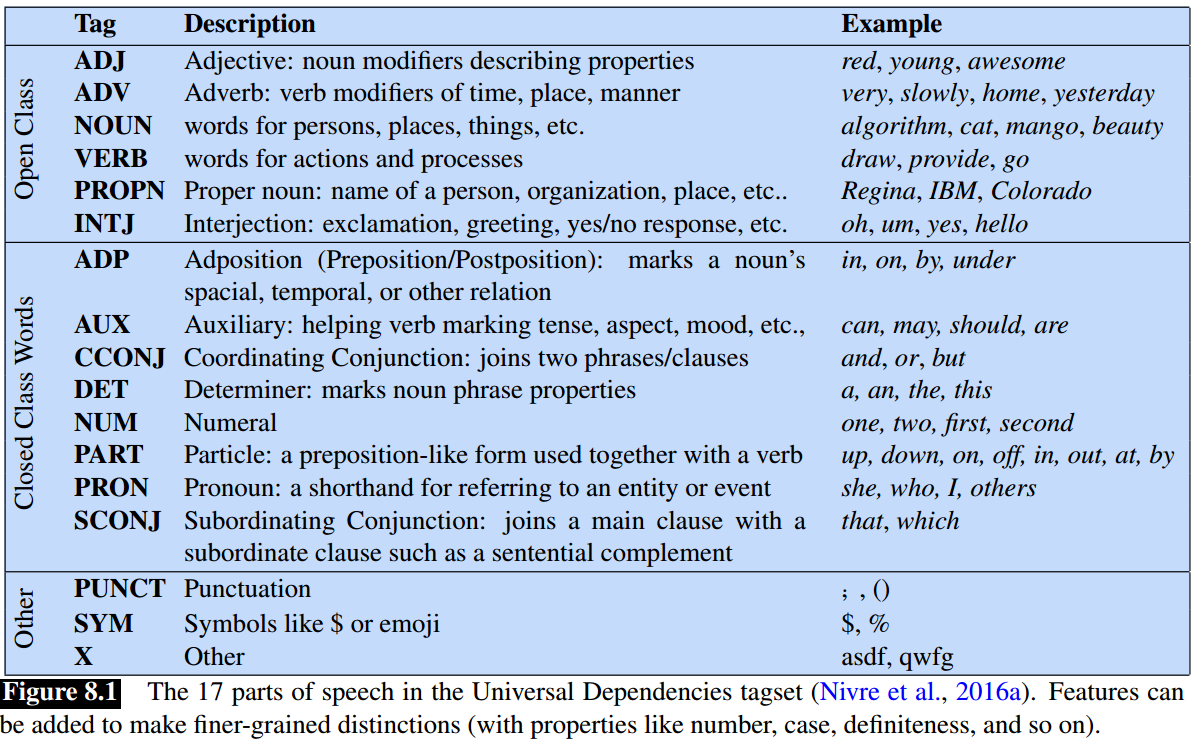
\includegraphics[scale = 0.4]{pos.png}}
\end{minipage}
\caption{\footnotesize{\textbf{The common part-of-speech in English}.}}
\label{fig: pos}
\end{figure}

\subsection{Word Classes in English}
The common part-of-speech tag can be seen in Figure \ref{fig: pos}. This includes \textbf{closed class} words and \textbf{open class} words: Closed classes are those with relatively fixed membership, such as prepositions—new prepositions are rarely coined. By contrast, nouns and verbs are open classes, since new names and actions are invented all the time. 

The open class words include:
\begin{itemize}
\item \textbf{noun (NOUN)}: words for person, things, places, etc. can be used for concrete terms, or abstract terms. Common nouns can be divided into \textbf{count nouns} or \textbf{mass nouns}. Count nouns can occur in the \emph{\textbf{singular}} and \emph{\textbf{plural}} (\emph{goat/goats}, \emph{relationship/relationships}) and can be \emph{counted} (one goat, two goats). Mass nouns are used when something is conceptualized as a \emph{homogeneous group}.
\item \textbf{verb (VERB)}: words for action and processes. English verbs have \emph{\textbf{inflections}} (\emph{\textbf{non-third-person-singular}} (eat), \textit{\textbf{third-person-singular}} (eats), \emph{\textbf{progressive}} (eating), \emph{\textbf{past participle}} (eaten)).
\item \textbf{adjective (ADJ)}: noun modifiers, describing noun
\item \textbf{adverb (ADV)}: verb modifiers, of manner, place, time etc. \textbf{Directional adverbs} or \textbf{locative adverbs} (\emph{home, here, downhill}) specify the direction or location of some action; \textbf{degree adverbs} (\emph{extremely, very, somewhat}) specify the extent of some action, process, or property; \textbf{manner adverbs} (\emph{slowly, slinkily, delicately}) describe the manner of some action or process; and \textbf{temporal adverbs} describe the time that some action or event
took place (yesterday, Monday).
\item \textbf{proper noun (PROPN)}: name of place, person etc. 
\item \textbf{interjection (INTJ)}: exclamation, greeting, yes/no response, etc. 
\end{itemize}

The closed class words include:
\begin{itemize}
\item \textbf{preposition/postposition (ADP)}: mark a noun's spacial, temporal, or other relation
\item \textbf{pronoun (PRON)}: a shorthand for referring to an entity or event such as \emph{I, me, he, she, you}.  \textbf{Wh-pronouns} (\emph{what, who, whom, whoever}) are used in certain question forms, or act as \textbf{complementizers} (\emph{Frida, who married Diego... }).
\item \textbf{auxiliary (AUX)}: such as \emph{can, make, need, may, should} etc. Auxiliary verbs mark \emph{semantic} features of a main verb such as its tense, whether
it is completed (aspect), whether it is negated (polarity), and whether an action is necessary, possible, suggested, or desired (mood). English auxiliaries include the
\textbf{copula verb} \emph{be}, the two verbs \emph{do} and \emph{have}, forms, as well as \textbf{modal verbs} used to mark the mood associated with the event depicted by the main verb: \emph{can} indicates ability or possibility, \emph{may} permission or possibility, \emph{must} necessity.
\item \textbf{determiner (DET)}: marks noun phrase properties such as \emph{this, that, a, an, the}.
\item \textbf{coordinating conjunction (CCONJ)}: such as \emph{and, but, however,}
\item \textbf{subordinating conjunction (SCONJ)}: such as \emph{which, where, that etc.} Subordinating conjunctions like \emph{that} \emph{which} link a verb to its argument in this way are also called \textbf{complementizers}
\item \textbf{numeral (NUM)}: numbers, \emph{one, two, three} etc.
\item \textbf{particle (PART)}: a proposition-like form used together with verb, \emph{down, up, off, on, at, by, out, in}. A particle resembles a preposition or an adverb and is used in combination with a verb. Particles often have \textbf{extended meanings} that aren’t quite the same as the prepositions they resemble, as in the particle \emph{over} in \emph{she turned the paper over}. A verb and a particle acting as \emph{a single unit} is called a \textbf{phrasal verb}. The meaning of phrasal verbs is often \textbf{non-compositional}—not predictable from the individual meanings of the verb and the particle.
\end{itemize} Closed class words are generally \textbf{function words} like \emph{of, it, and, or you}, which tend to be very short, occur frequently, and often have \emph{structuring} uses in grammar.

Figure \ref{fig: pos_tag} shows the symbol of part-of-speech tag from Penn Treebank \citep{jurafsky2014speech}. 
\begin{figure}
\begin{minipage}[t]{1\linewidth}
  \centering
  \centerline{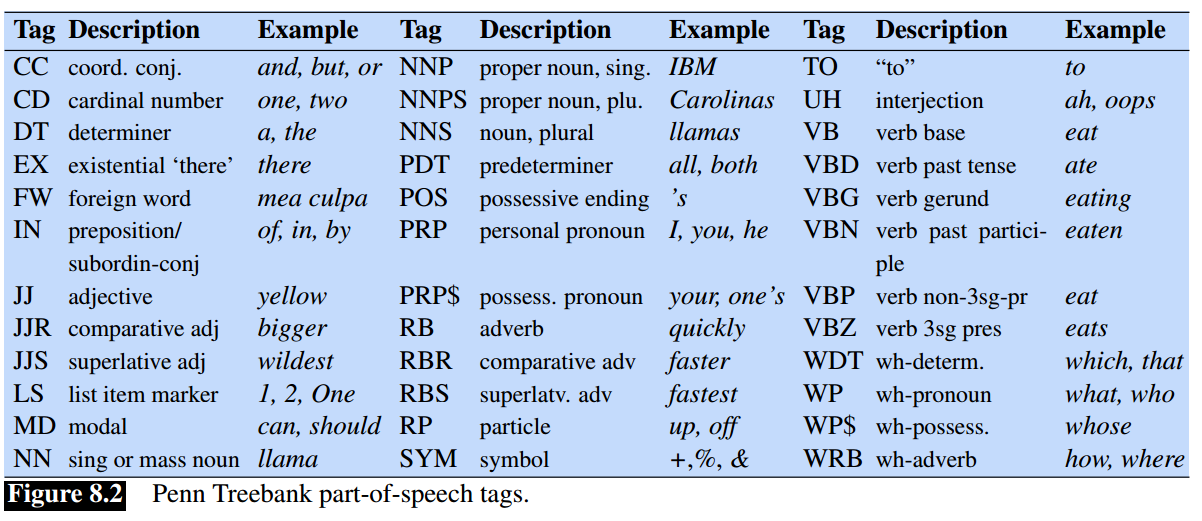
\includegraphics[scale = 0.4]{pos_tag.png}}
\end{minipage}
\caption{\footnotesize{\textbf{The part-of-speech tag in Penn Treebank}.}}
\label{fig: pos_tag}
\end{figure}

\section{Part-of-speech tagging}
\textbf{Part-of-speech tagging} is the process of assigning a part-of-speech to each word in a text. The input is a sequence $x_1, x_2, \ldots x_n$ of (tokenized) words and a tagset, and the output is a sequence $y_1, y_2, \ldots, y_n$ of tags, each output $y_i$ corresponding exactly to one input $x_i$, as shown in the intuition in Figure \ref{fig: pos_tag_example}. 

Tagging is a \textbf{disambiguation} task; words are ambiguous — have more than one possible part-of-speech — and the goal is to find the correct tag for the situation. The goal of POS-tagging is to resolve these ambiguities, choosing the proper tag for the context (i.e. \textbf{ambiguity resolution}). Nonetheless, many words are easy to disambiguate, because their different tags aren’t equally likely. For example, "\emph{a}" can be a determiner or the letter \emph{a}, but the determiner sense is much more likely. 

This idea suggests a useful \textbf{baseline}: given an ambiguous word, choose the tag which is most \textbf{frequent} in the training corpus. This is a key concept:

\emph{\textbf{Most Frequent Class Baseline}: Always compare a classifier against a baseline at least as good as the most frequent class baseline (assigning each token to the class it occurred in most often in the training set).}

The most-frequent-tag baseline has an accuracy of about $92\%$. The standard technique behinds POS tagging is \textbf{sequence labeling}, i.e. for an input sequence of texts, output a sequence of labels, each for a text. 

\begin{figure}
\begin{minipage}[t]{1\linewidth}
  \centering
  \centerline{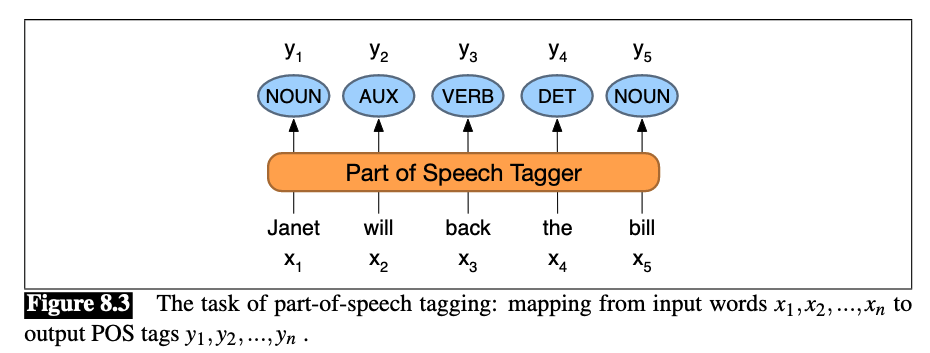
\includegraphics[scale = 0.4]{pos_tag_example.png}}
\end{minipage}
\caption{\footnotesize{\textbf{The part-of-speech tagging process}.}}
\label{fig: pos_tag_example}
\end{figure}

\section{Named Entities and Named Entity Tagging}
A \textbf{named entity} is, roughly speaking, anything that can be referred to with a proper name: a \emph{person}, a \emph{location}, an \emph{organization}. The task of \textbf{named entity recognition (NER)} is to find \emph{spans} of text that constitute proper names and tag the type of the entity. \textbf{Four} entity tags are most \textbf{common}: \textbf{PER (person)}, \textbf{LOC (location)}, \textbf{ORG (organization)}, or \textbf{GPE (geo-political entity)}. However, the term named entity is commonly extended to include things that aren’t entities per se, including \textbf{dates},
\textbf{times}, and other kinds of \textbf{temporal expressions}, and even \textbf{numerical expressions} like prices. Figure \ref{fig: ner_example} shows name entities in a paragraph. 

\begin{figure}
\begin{minipage}[t]{1\linewidth}
  \centering
  \centerline{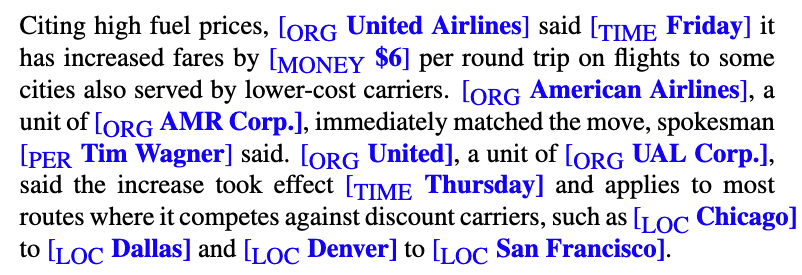
\includegraphics[scale = 0.4]{ner_example.png}}
\end{minipage}
\caption{\footnotesize{\textbf{An example of name entities in a paragraph}.}}
\label{fig: ner_example}
\end{figure}

Named Entity Recognition can be used as pre-processing steps for \emph{sentiment analysis}, \emph{question answering} as well as learning \emph{semantic representations} such as event extraction and relationship inference. 

NER is more challenging than POS tagging. For POS tagging, each word has only one part-of-speech tag but for NER, there is a \emph{segmentation} problem. The task of NER is to find and label the \emph{span} of text. The ambiguity of segmentation brings additional challenge: we need to decide what’s an entity and what isn’t, and where the boundaries are. 

The standard approach that convert the span-recognition to sequence labeling is \textbf{BIO tagging} \citep{jurafsky2014speech}. This is a method that allows us to treat NER like a word-by-word sequence labeling task, via \textbf{tags} that \emph{capture both the boundary and the named entity type}. Similarly, there are \textbf{IO tagging} and \textbf{BIOES tagging}.

\begin{figure}
\begin{minipage}[t]{1\linewidth}
  \centering
  \centerline{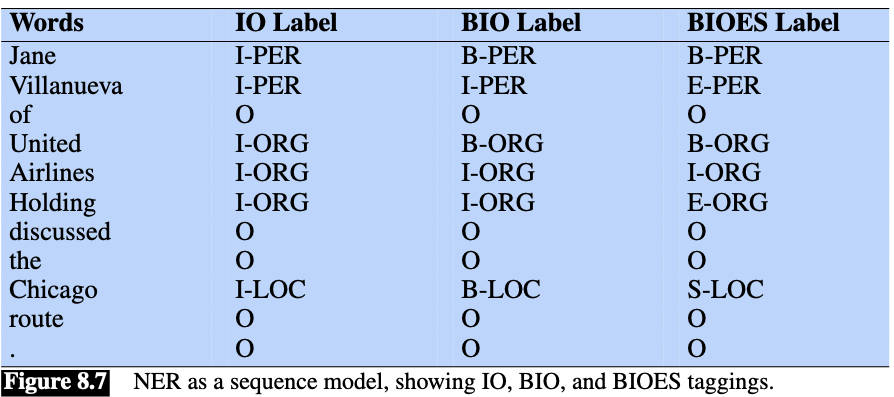
\includegraphics[scale = 0.4]{bio_tagging.png}}
\end{minipage}
\caption{\footnotesize{\textbf{BIO, IO and BIOES tagging for NER}.}}
\label{fig: ner_bio_example}
\end{figure}

In BIO tagging we label any token that begins a span of interest with the label \textbf{B}, tokens that occur inside a span are tagged with an \textbf{I}, and any tokens outside of any span of interest are labeled \textbf{O}. There is only \emph{one} \textbf{O} tag to indicate not a named entity. On the other hand, we can have distinct \textbf{B} and \textbf{I} for each named entity type, i.e. \textbf{B-PER}, \text{I-PER}, \text{B-ORG}, \text{I-ORG} etc. For $n$ distinct named entity types, there are $2n + 1$ distinct tags. BIO tagging can represent exactly the same information as the bracketed notation, but has the advantage that we can represent the task in the same simple sequence modeling way as part-of-speech tagging. In BIOES tagging, we add \textbf{E} tag for end of a span, and a span tag \textbf{S} for a span consist of only one word.  

A \textbf{sequence labeler} (HMM, CRF, RNN, Transformer, etc.) is trained to label each token in a text with tags that indicate the presence (or absence) of particular kinds of named entities.

\newpage
\bibliographystyle{plainnat}
\bibliography{book_reference.bib}
\end{document}